\chapter{Cómo arreglar una canción}
\label{cap:comoArreglarCancion}
Hacer un arreglo de una canción consiste en utilizar una idea musical, una composición o una canción entera para crear una canción nueva.

En nuestro caso vamos a usar un motivo o idea musical para arreglar una canción que funcione como música para un videojuego. Hay muchas formas de abordar esto, y como es común en la música y el arte, no hay una verdad absoluta.

Por nuestra parte, priorizamos que el arreglo funcione pero sea rico y variado, con varias secciones y sonidos posibles, de manera que dos generaciones distintas no sean nunca iguales. Bajo esta premisa, hemos definido una serie de normas para la estructura y timbres de la canción, que se generarán de manera pseudoaleatoria siguiendo dichas normas.


\section{Temáticas}
\label{sec:tematicas}

Para lograr que una canción suene a una temática en concreto o transmita un sensación son importantes varios factores, entre ellos los timbres, el tempo de la canción o la tonalidad.

Tanto para abordar algunas temáticas como para la idea de separar en temáticas teniendo en cuenta los factores mencionados, nos hemos inspirado en los vídeos de YouTube  del canal "Ludofonia"  (\cite{LudofoniaDesierto}).

La mayoría de adaptaciones según el tema se realizan en Reaper (Sección \ref{sec:reaper}) mediante el uso de plugins, efectos, selección de tempo y selección de la escala de la canción.

A continuación, desglosaremos cada temática disponible en la herramienta, explicando de qué forma hemos enfocado cada una:

\begin{itemize}
    \item \textbf{Pradera}: Canciones en modo lidio con un tempo de en torno a 120BPM. Usamos timbres de pianos, guitarras y algunos instrumentos de cuerda, junto con un bajo eléctrico y distintas cajas de ritmos para la batería.
    \item \textbf{Piano}: Usamos la tonalidad original del MIDI cargado o generado por la herramienta. El BPM es aleatorio dentro de un amplio rango. A la hora de hacer el arreglo sólo tenemos dos pistas sonando simultáneamente como máximo, y todas las pistas tienen el mismo instrumento virtual de piano.
    \item \textbf{Desierto}: Usamos el modo frigio para esta temática, además de usar varios timbres característicos como sitars, flautas, guitarras, percusiones, palmas, etc. Para más información ver \cite{LudofoniaDesierto}.
    \item \textbf{Nieve}: Modo dórico con BPM lento. Sonidos suaves y agradables, timbres característicos como campanas o kalimbas.
    \item \textbf{Pirata}: Modo mixolidio y BPM elevado. Timbres característicos como acordeones, violines, percusiones variadas, guitarras, etc. Algo muy importante mencionado en el vídeo de YouTube del canal "Ludofonia" sobre la música pirata (\cite{LudofoniaPiratas}) es que la melodía suele ir en 3/4 o atresillada, algo hemos logrado mediante el uso del plugin \textit{BlueArp} (Sección \ref{subsubsec:bluearp}). 
    \item \textbf{Selva}: La mayoría de pistas cargan percusiones además de otros sonidos típicos de jungla como las marimbas. Para esta temática nos ayudamos del exotismo del modo frigio, además, el tempo utilizado es bastante rápido. Para más información ver \cite{LudofoniaJungla}.
    \item \textbf{Épico}: Varios instrumentos orquestales, en su mayoría de cuerda y viento metal. Usamos timbales para la percusión. Usamos el modo mixolidio.
    \item \textbf{Tenebroso}: Modo locrio, sonidos no muy agradables sonando en varias pistas. Para más información ver \cite{LudofoniaTetrico}.
    \item \textbf{Agua}: Modo mixolidio y BPM lento. Sonidos suaves y algunos efectos de agua generados con sintetizadores. Para más información ver \cite{LudofoniaAgua}.
    \item \textbf{Asiático}: Modo lidio, mezcla entre  instrumentos tradicionales asiáticos y una batería moderna junto a un bajo eléctrico.
    \item \textbf{Rock}: Modo dórico. Cargamos varias guitarras eléctricas con amplificadores con distorsión junto con una batería de rock.
    \item \textbf{Pop}: Usamos la tonalidad original del MIDI cargado o generado por la herramienta. Varios instrumentos de música pop actual como guitarras, pianos, sintetizadores, etc.
    \item \textbf{Tecno}: Usamos la tonalidad original del MIDI cargado o generado por la herramienta. Percusión electrónica golpeando el bombo a negras haciendo un efecto de \textit{sidechain}\footnote{\url{https://es.wikipedia.org/wiki/Sidechain}} sobre varios sintetizadores (este efecto de \textit{sidechain} lo simulamos con una envolvente).
\end{itemize}


\section{Las partes fundamentales de una producción}
\label{sec:fundamentos-producccion-musical}
El proceso de producir una canción es un proceso complejo y bastante creativo, pero podemos reducirlo a una serie de normas básicas con el fin de simplificarlo.

Proponemos hacer producciones a partir de los siguientes cuatro elementos fundamentales: La melodía, el acompañamiento, el bajo y la batería.

%TODO: esto bien
\begin{itemize}
    \item \textbf{Melodía}: Elemento protagonista y más distintivo de una canción. Especificado la Sección \ref{sec:como-generamos-melodias}.
    \item \textbf{Armonía}: Acompaña a la melodía, generalmente formando acordes. Especificado en la Sección \ref{sec:arm:armonia}.
    \item \textbf{Bajo}: Encargado de las frecuencias graves de una canción. Especificado en la Sección \ref{sec:lineas-de-bajo}.
    \item \textbf{Batería}: Encargado de llevar el ritmo en una canción. Especificado en la Sección \ref{sec:generacion-percusion}.
\end{itemize}


\section{Secciones}
\label{sec:secciones}

Estructuramos la canción en un máximo de 8 secciones, las cuales tienen una duración de 8 compases cada una. Lo ideal para que una canción no se vuelva repetitiva es añadir o quitar elementos cada poco tiempo, siendo lo más común cada 8 compases.

El usuario puede, desde Reaper, eligir si quiere renderizar la canción entera de 8 secciones, o seleccionar un rango se secciones para renderizar únicamente esas, ya que mientras sean secciones enteras y no se corten a la mitad, \textit{loopearan} de forma correcta sea cual sea la selección.


\section{Arreglo}
\label{sec:arreglo}

Generamos una matriz de booleanos de 7x8 la cuál rellenamos de maneras aleatoria, y que posteriormente corregimos siguiendo unas normas:

\begin{itemize}

\item No puede haber dos pistas de acompañamiento sonando simultáneamente.
\item En la primera sección no puede haber más de tres instrumentos principales (Sección \ref{subsec:instrumentos-secundarios}) sonando a la vez.
\end{itemize}

En la Figura \ref{fig:ArregloReaper} podemos ver una captura de pantalla que muestra un arreglo que la herramienta ha cargado en Reaper. 

\begin{figure}[h]
    \centering
    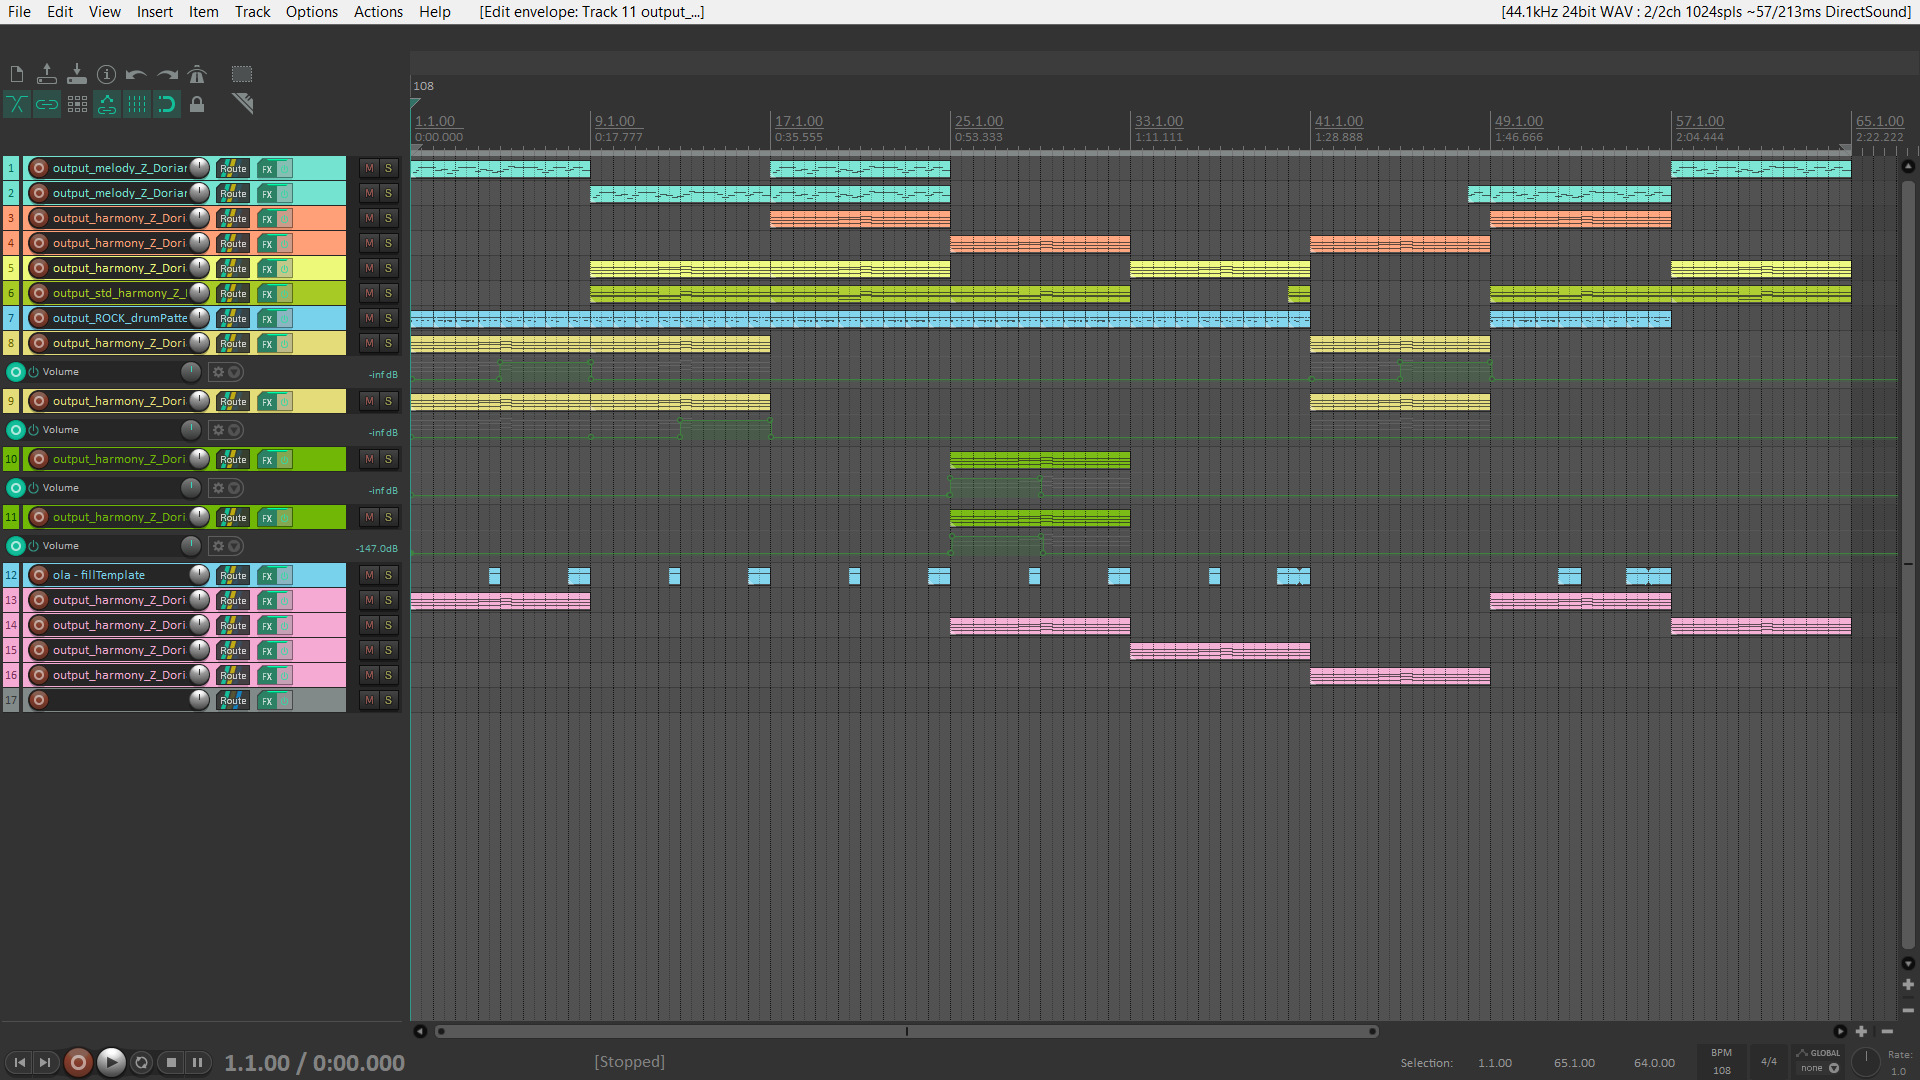
\includegraphics[width = 0.9\textwidth]{Imagenes/Bitmap/ArregloReaper.png}
    \caption{Arreglo generado en Reaper}
    \label{fig:ArregloReaper}
\end{figure}

\section{Pistas}\label{sec:pistas}

Dependiendo de la temática (Sección \ref{sec:tematicas}) de la canción, la herramienta cargará en Reaper varios efectos (Sección \ref{subsec:plugin}) por pista, la mayoría son genéricos dependiendo de la temática y pista concreta, pero el instrumento que interpretará el MIDI(Sección \ref{subsec:que-es-midi}) cargado se seleccionará de manera aleatoria de entre unos plugins vst (Sección \ref{subsec:plugins-utilizados}) seleccionados por nosotros.



\section{Complejidad de las melodías}

Una vez tenga una melodía, el usuario puede determinar, desde la ventana de la aplicación de la herramienta, la complejidad con la que se cargarán las melodías en Reaper. Hay tres complejidades:
\begin{itemize}
    \item \textbf{Estándar}: Cargamos el MIDI de melodía entero en Reaper, por tanto la melodía se repetirá cada 8 compases, como se puede ver en la Figura \ref{fig:ComplejidadEstandar}. 

\begin{figure}[h]
    \centering
    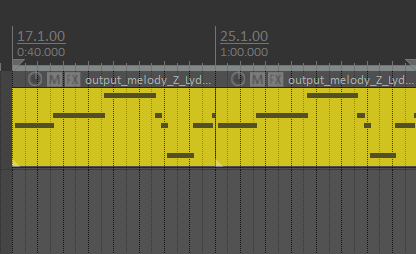
\includegraphics[width = 0.5\textwidth]{Imagenes/Bitmap/ComplejidadEstandar.png}
    \caption{Ítems MIDI en complejidad estándar}
    \label{fig:ComplejidadEstandar}
\end{figure}
    \item \textbf{Repetitiva}: 
La repetición en la melodía es clave para que la canción sea predecible y sea fácil de recordar. En esta complejidad las melodías se repiten cada dos compases. Para lograr esto, troceamos el MIDI de melodía original proporcionado en cuatro partes y las cargamos de forma pseudoaleatoria, como se puede ver en la Figura \ref{fig:ComplejidadRepetitiva}.

\begin{figure}[h]
    \centering
    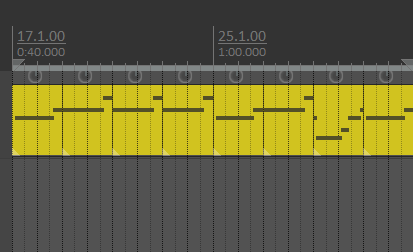
\includegraphics[width = 0.5\textwidth]{Imagenes/Bitmap/ComplejidadRepetitiva.png}
    \caption{Ítems MIDI en complejidad repetitiva}
    \label{fig:ComplejidadRepetitiva}
\end{figure}

    \item \textbf{Súper repetitiva}: Similar a la complejidad anterior, pero esta vez con ítems MIDI todavía más cortos. Se repite la secuencia de ítems dos veces por cada 8 compases, como se puede ver en la Figura \ref{fig:ComplejidadSuperRepetitiva}.

\begin{figure}[h]
    \centering
    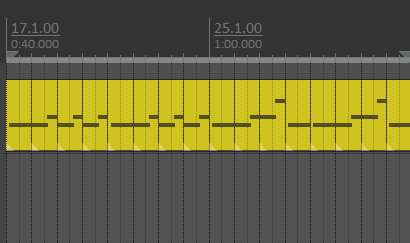
\includegraphics[width = 0.5\textwidth]{Imagenes/Bitmap/ComplejidadSuperRepetitiva.png}
    \caption{Ítems MIDI en complejidad súper repetitiva}
    \label{fig:ComplejidadSuperRepetitiva}
\end{figure}

\end{itemize}

\section{Línea de bajo}\label{sec:lineas-de-bajo}
Al comienzo del desarrollo de la herramienta implementamos un generador de líneas de bajo que creaba, a partir de una armonía dada, una melodía monofónica para ser interpretada por el bajo, usando principalmente la nota más grave de cada acorde (que puede no ser la fundamental, ya que la armonía puede tener inversiones de acordes). Este generador es similar al generador de percusión (Sección \ref{subsec:generacion-percusion-propia}) pero simplificado.

Este algoritmo tenía algunas limitaciones y a la hora de ampliarlo para añadir variedad, decidimos optar por una alternativa más cómoda y flexible.

En la versión actual de la herramienta, cargamos la armonía (Sección \ref{sec:arm:cuestion}) (sin inversiones) en Reaper en la pista de bajo y utilizamos el plugin \textit{BlueArp} (Sección \ref{subsubsec:bluearp}) para interpretar la línea de bajo usando principalmente la nota fundamental del acorde y en ocasiones el resto de notas de dicho acorde.

%TODO: explicar y referenciar estas imagenes

\begin{figure}[h]
    \centering
    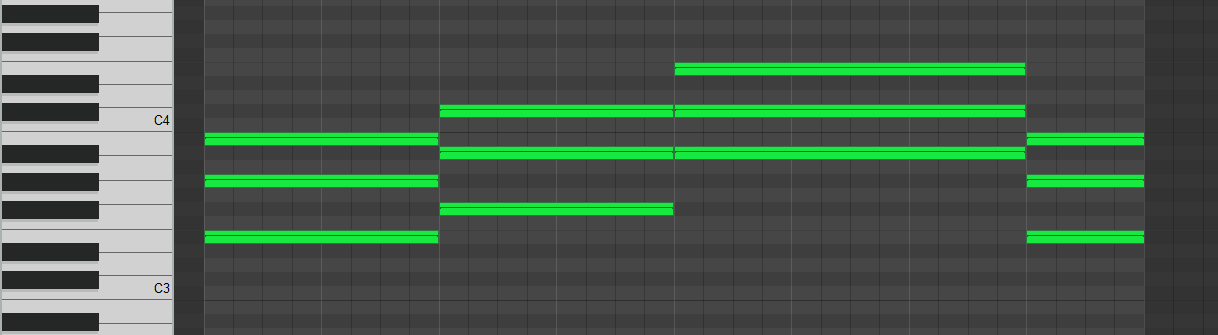
\includegraphics[width = 0.5\textwidth]{Imagenes/Bitmap/LineaDeBajo1.png}
    \caption{Progresión de acordes sin inversión}
    \label{fig:LineaDeBajoAcordes}
\end{figure}

\begin{figure}[h]
    \centering
    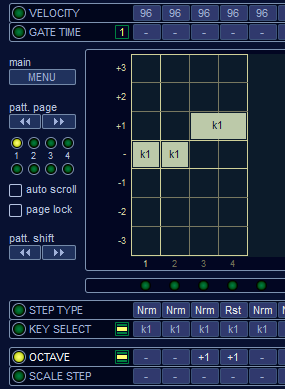
\includegraphics[width = 0.3\textwidth]{Imagenes/Bitmap/LineaDeBajo2.png}
    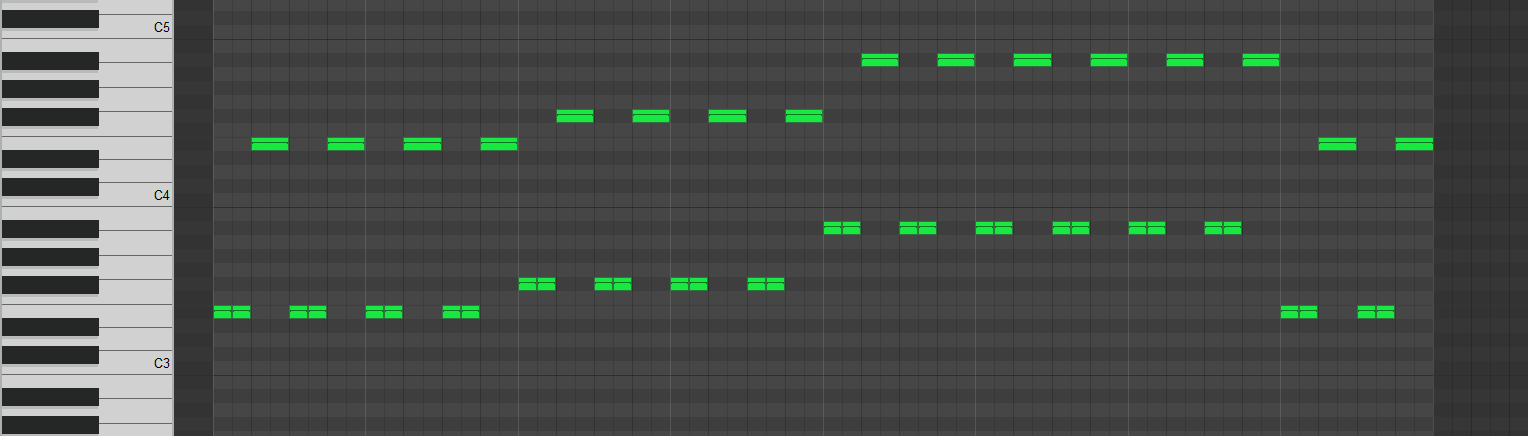
\includegraphics[width = 0.5\textwidth]{Imagenes/Bitmap/LineaDeBajo3.png}
    \caption{Configuración de \textit{BlueArp} y línea de bajo resultante}
    \label{fig:LineaDeBajo1}
\end{figure}

\begin{figure}[h]
    \centering
    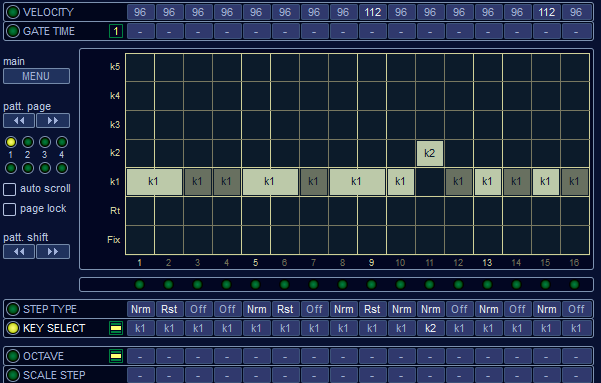
\includegraphics[width = 0.3\textwidth]{Imagenes/Bitmap/LineaDeBajo4.png}
    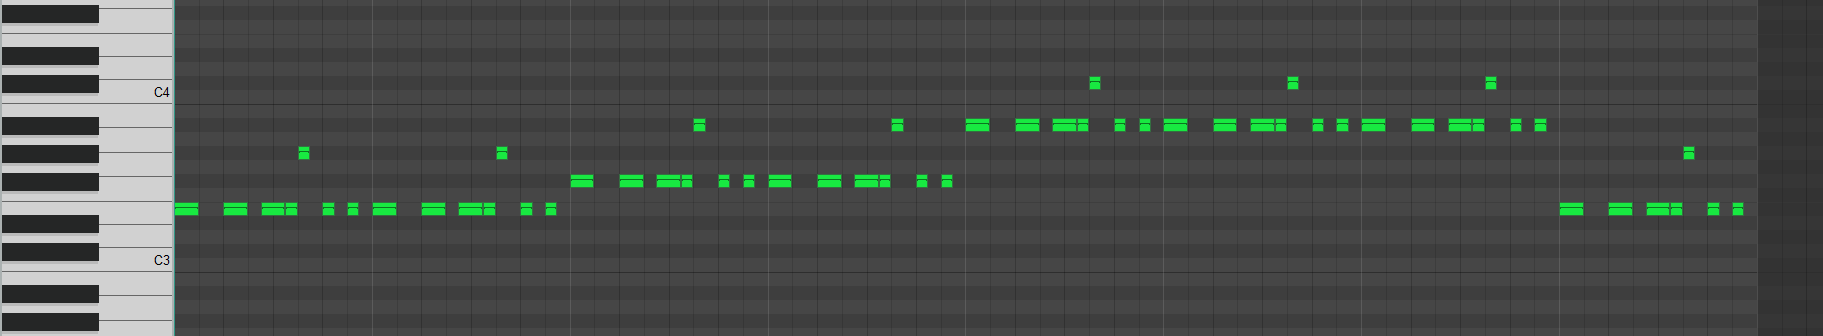
\includegraphics[width = 0.5\textwidth]{Imagenes/Bitmap/LineaDeBajo5.png}
    \caption{Configuración de \textit{BlueArp} y línea de bajo resultante}
    \label{fig:LineaDeBajo2}
\end{figure}


\section{Arreglos de batería}
Dependiendo del estilo de la canción (Sección \ref{sec:tematicas}), se genera cada cuatro compases de forma aleatoria un estilo de batería o género musical de entre hasta tres posibles. Se cargan alternando las 3 variaciones distintas que nos proporciona el generador de percusión (Sección \ref{subsec:generacion-percusion-propia}) formando un patrón calculado de forma aleatoria una única vez. Por ejemplo si el patrón calculado es ABAC, patrón típico de batería, cargaríamos el MIDI correspondiente al ritmo A, de longitud de un compás, a continuación el ritmo B, de nuevo el A y después el C, y repetiríamos el mismo patrón ABAC durante toda la canción.

\section{\textit{Ear candy}}
\label{sec:ear-candy}
El \textit{ear candy} en la producción musical consiste en añadir pequeños elementos a una canción para volverla más interesante, que no son imprescindibles para la canción, pero que captan la atención del oyente o ayudan a dar coherencia a la mezcla. Podríamos decir que el \textit{ear candy} es la guinda del pastel en una canción.

A partir del arreglo inicial, nuestro programa sigue unas reglas para añadir varios tipos de \textit{ear candy}: transiciones, \textit{drum fills} y sonidos adicionales que enriquecen la mezcla final:


\begin{itemize}

\item Transiciones: cuando una sección contiene un número determinado de instrumentos sonando simultáneamente y la sección siguiente contiene al menos un instrumento más, se añade un \textit{riser} formado a partir de un sonido aleatorio con mucha reverb que va aumentando en volumen según nos acercamos al cambio de sección. En el caso contrario, es decir, que haya varios elementos en una sección y en la siguiente al menos 2 elementos menos, se agrega un \textit{downriser}, que no es más que un sonido reverberado también pero esta vez decreciente en volumen.

\item \textit{Drum fill}: (Sección \ref{subsubsec:generacion-drum-fills}) Cuando va a entrar un instrumento de batería en la próxima sección, y sólo si no hay un \textit{riser} colocado para la transición, se coloca un \textit{drum fill} que sonando sin otros instrumentos de batería, funciona como un ritmo de introducción al patrón de batería. Adicionalmente, cada 4 compases de percusión, colocamos un \textit{drum fill} que suena a la vez que el ritmo principal para añadirle movimiento, siendo de mayor duración en los compases múltiplos de 8 y cuanto más avanzados en la canción estemos.

\item  Entrada adelantada de sonidos: Si entre dos secciones no hay ningún elemento común, uno de los elementos adelanta su entrada para que el cambio no sea muy brusco. Al elegir instrumento para hacer esto, tiene prioridad el instrumento de bajo. Si no hay bajo presente, será la melodía o el acompañamiento el que resuelva esto, en ese orden de prioridad.

\item  Sonidos adicionales: Si en una sección no hay muchos sonidos presentes, se agregarán de forma aleatoria algunos sonidos (con más o menos protagonismo en la mezcla) a lo largo de la sección.

\end{itemize}



\subsection{Instrumentos principales}
\label{subsec:instrumentos-principales}
Estos instrumentos son los que harán sonar la matriz del arreglo(Sección \ref{sec:arreglo}). Cubren las necesidades básicas de toda producción (Sección \ref{sec:fundamentos-producccion-musical}) y son los siguientes:


%TODO: Hacer esto más homogéneo y ponerle referencias a una figura de ejemplo.
\begin{itemize}
\item 2 pistas de melodía: una de ellas una octava por encima de la otra. En esta pista van los MIDIs de melodía (Sección \ref{sec:como-generamos-melodias})
\item 2 pistas de acompañamiento. No pueden sonar al mismo tiempo, ya que los arpegios generados pueden sonar mal en conjunto. Estas pistas van acompañadas de un arpegiador que hará que en ocasiones los acordes sean arpegiados o tocados con otro ritmo distinto al del MIDI. Estas pistas cargan el MIDI de armonía (Sección \ref{sec:arm:cuestion})
\item Una pista de pads. Esta pista carga el MIDI de armonía (Sección \ref{sec:arm:cuestion}), por lo que interpreta los acordes de la canción. Cuando suena sin el acompañamiento hace la propia función de acompañar a la melodía algo más en segundo plano, y cuando suena a la vez que el acompañamiento complementa el sonido de este.
\item Una pista de bajo. Esta pista carga el MIDI de armonía (Sección \ref{sec:arm:cuestion}) pero esta vez sin inversiones (Sección \ref{sec:arm:acordes})). Esto es porque en el bajo generalmente queremos una melodía monofónica con las notas fundamentales de cada acorde, y necesitamos que la fundamental sea la nota más grave porque le metemos un arpegiador \textit{BlueArp}(Sección \ref{subsubsec:bluearp}) para tocar o bien únicamente esa nota, o un arpegio o una línea de bajo.
\item Una pista de batería. Esta pista carga varios MIDIs de batería (Sección \ref{subsec:generacion-percusion-propia}) dependiendo de la temática de la canción (Sección \ref{sec:tematicas})
\end{itemize}


%TODO: esta sección y la anterior fusionarla con el resto del capítulo. Ejemplo: hablo de las líneas de bajo y digo, apoyándome en el ejemplo, cargo una pista de bajo con estas características. Así con todo.
\subsection{Instrumentos secundarios}
\label{subsec:instrumentos-secundarios}
En estas pistas se cargarán los instrumentos son los que generarán los sonidos de los \textit{ear candy} (Sección \ref{sec:ear-candy}) a partir de la disposición del arreglo. Son sonidos que no acaparan el protagonismo, más bien se encuentran en un segundo plano y es fácil que no te des cuenta de que están ahí, pero hacen una diferencia significativa a la hora de dar cohesión y dinamismo a una canción. Son los siguientes:


\begin{itemize}
\item 2 pistas de \textit{uprisers}. Cargan el MIDI de acompañamiento para crear transiciones usando un sonido reverberado que deja de sonar al entrar la nueva sección. Sólo puede sonar una simultáneamente, son dos para añadir variedad.

\item 2 pistas de \textit{downrisers}. Al igual que los uprisers, cargan el MIDI de acompañamiento pero esta vez para generar una bajada, usando una Reverb con menos ataque (alcanza más volumen antes) que baja de volumen progresivamente.

\item Una pista de \textit{drum fills} (Sección \ref{subsubsec:drum-fills}). Suenan de forma simultánea a las baterías o cuando va a entrar una sección con batería y no estaba sonando en la sección actual. Carga un MIDI especial que tiene marcadas las notas de bombo, caja y dos platillos, que serán interpretados por el arpegiador \textit{BlueArp}(Sección \ref{subsubsec:bluearp}) y con el humanizador(Sección \ref{subsubsec:humanizador}) configurado con algo de aleatoriedad en el pitch, lo que en instrumentos de batería significa que sonarán distintos golpes (cajas, platillos, toms, palmas) cada vez.

\item 4 pistas de sonidos puntuales (Sección \ref{sec:ear-candy}). Cargan el MIDI de la armonía y suenan al menos dos veces por sección (Sección \ref{sec:secciones}) durante un periodo corto de tiempo si la sección cumple los requisitos planteados en la sección de \textit{ear candy}. Usan un arpegiador  para interpretar una melodía tocando las notas presentes en el acorde y llevan un efecto de delay creado con el plugin \textit{CRMBL} Sección \ref{subsubsec:delay}.
\end{itemize}

